\documentclass[aspectratio=169]{beamer}
\usepackage{fontawesome}
\usepackage{hyperref}
\usepackage{url}
\usetheme{Madrid}
\usecolortheme{sidebartab}
\usefonttheme{professionalfonts}
\urlstyle{same}

\title{Ansible for Network Automation}
\subtitle{Ansible Variables and Folder Structure}
\date{}
\author{Josh VanDeraa}

\begin{document}
% \frame{\titlepage}
\begin{frame}
  \maketitle
  \footnotesize
  \faTwitter vanderaaj \hfill \faGithub jvanderaa \hfill \faSlack jvanderaa
\end{frame}

\begin{frame}
  \frametitle{Session Overview}
  At the end of this session you will:
  \begin{itemize}
    \item <2-> Reviewed a common folder structure for use with Ansible
    \item <3-> Understand where you can define variables for use in Ansible
    \begin{itemize}
      \item <3-> all.yml
      \item <4-> group\_vars folder
      \item <5-> host\_vars folder
      \item <6-> Importing variables from another file
      \item <7-> Accessing variables from other devices
    \end{itemize}
  \end{itemize}
\end{frame}

\begin{frame}
  \frametitle{Directory Structure}
  \begin{center}
    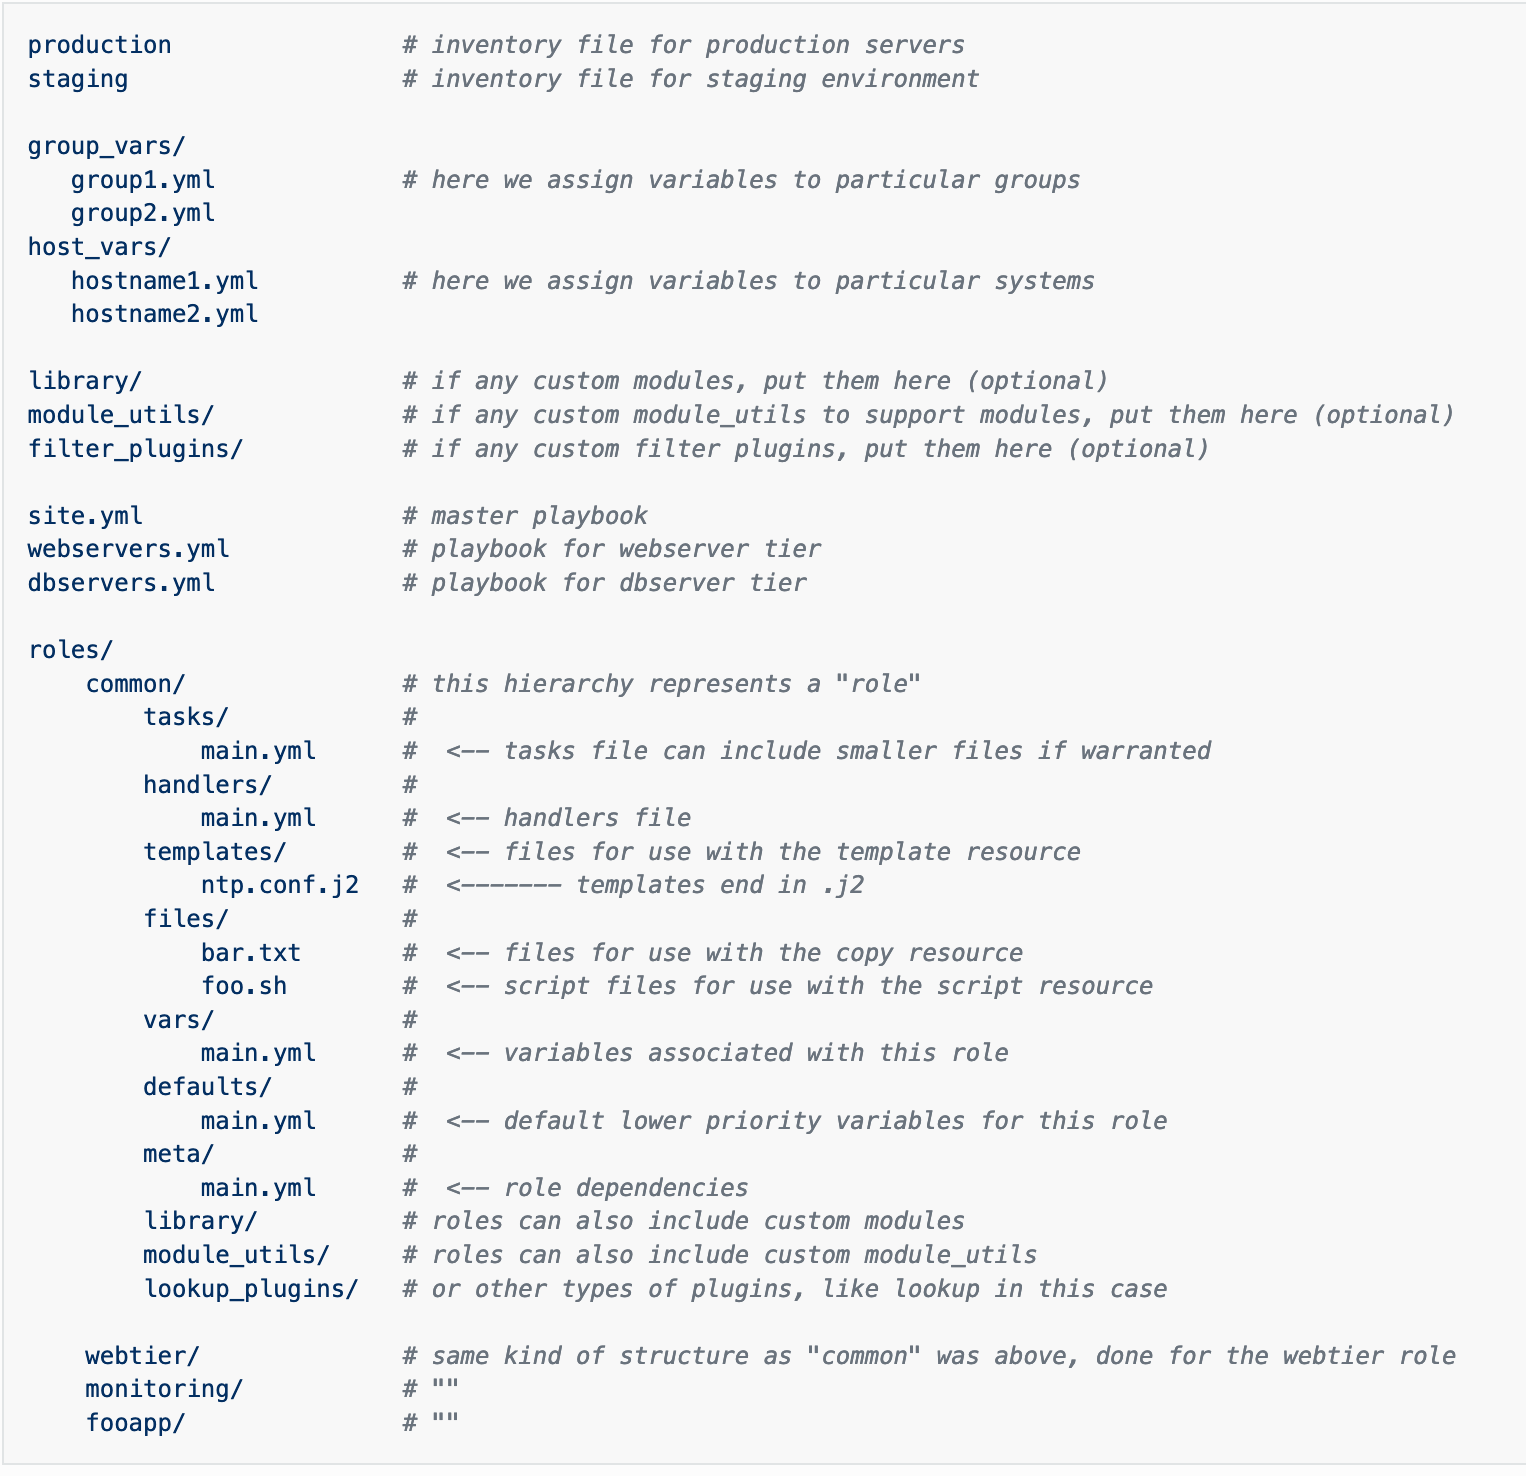
\includegraphics[height=\textheight]{assets/directory_layout.png}    
  \end{center}  
\end{frame}
  
\begin{frame}
  \frametitle{DEMO!}
  \begin{columns}
  \begin{column}{0.3\textwidth}
    \Huge
    \begin{center}
      \faDesktop 
      \hspace{.5cm}
      \faRocket     
    \end{center}
  \end{column}
  \begin{column}{0.7\textwidth}
    \huge 
      Let's take a look!
      \begin{itemize}
        \item Directory Structure
        \item Variable Inheritance
      \end{itemize}
  \end{column}
  \end{columns}
\end{frame}

% THIS IS THE ENDING SLIDE... NEEDS TO GET UPDATED!!!!!
\begin{frame}
  \frametitle{Summary}
    To review what we accomplished today:
    \begin{itemize}
      \item <2-> Reviewed a common folder structure for use with Ansible
      \item <3-> Understand where you can define variables for use in Ansible
      \begin{itemize}
          \item <3-> all.yml
          \item <4-> group\_vars folder
          \item <5-> host\_vars folder
          \item <6-> Importing variables from another file
          \item <7-> Accessing variables from other devices
      \end{itemize}
    \end{itemize}
\end{frame}

\begin{frame}
    \frametitle{Contact}
    \huge
    \begin{center}
      \url{https://packetpushers.slack.com}
    \end{center}
    \begin{center}
      \normalsize
      \faSlack \hspace{.1cm}jvanderaa  
    \end{center}
  \end{frame}

\end{document}